% Define a common style for blocks - this style is labeled "myBlock"
\tikzstyle{myBlock}=[draw, fill=blue!30!white, minimum size=0.5in, node distance=1.5in]

% Import required TikZ libraries
\usetikzlibrary{arrows.meta}

% Define common style for path lines - this style is labeled "myPath"
\tikzstyle{myPath} = [-{Latex[length=2mm,width=2mm]}, line width=0.4mm]

\begin{figure}[H]
\centering
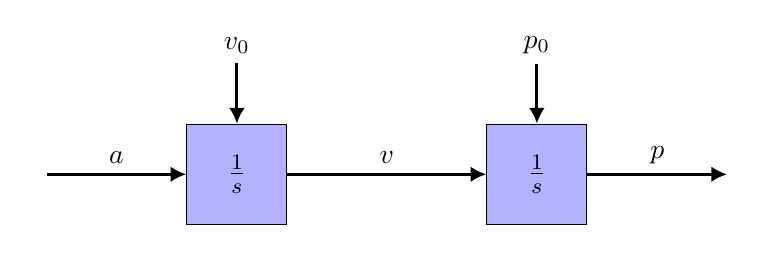
\begin{tikzpicture}
   % Draw initial node denoted by "v" label
   \node[myBlock] (v) {\large$\frac{1}{s}$};
   % Draw second node, "p" label, with location relative to node "a"
   \node[myBlock] (p) [right of=v] {\large$\frac{1}{s}$};

   % Draw initial condition inputs with labels "v0" and "p0"
   \node (v0) [above of=v, yshift=0.25in] {$v_0$};
   \node (p0) [above of=p, yshift=0.25in] {$p_0$};

   % Draw lines from initial conditions to blocks
   \draw[myPath] (v0) -- (v);
   \draw[myPath] (p0) -- (p);

   % Draw line between each of the blocks
   \draw[myPath] (v) -- (p) node [midway, above] {$v$};

   % Create dummy nodes to with no content
   \node[node distance=1in] (dummy_v) [left of=v] {};
   \node[node distance=1in] (dummy_p) [right of=p] {};

   % Draw lines from dummy nodes to blocks
   \draw[myPath] (dummy_v) -- (v) node [midway, above] {$a$};
   \draw[myPath] (p) -- (dummy_p) node [midway, above] {$p$};
\end{tikzpicture}
\caption{Example Block Diagram Using TikZ Package} 
\label{fig:block_diagram}
\end{figure}